\chapter{Experimentos}
\label{experimentos}

Os operadores propostos nesta pesquisa podem ser compostos de diferentes formas, 
construindo diversas heurísticas que podem encontrar soluções distintas para 
\ac{tmap}. Assim, este capítulo tem dois objetivos. O primeiro é encontrar as 
melhores combinações de operadores. O segundo é comparar as heurísticas que 
obtiveram melhores resultados com abordagens propostas por outros autores.

Os operadores descritos neste trabalho foram implementados na linguagem de 
programação Java\footnote{\url{http://java.com/pt_BR/}}. A principal razão para 
a adoção desta linguagem foi o \textit{Simple Patrol}, simulador da \ac{tmap}, 
desenvolvido pelo grupo de pesquisa sobre Patrulha Multiagente da Universidade 
Federal Rural de Pernambuco, utilizado para realizar os experimentos desta 
pesquisa. Os operadores foram desenvolvidos de forma compatível com a biblioteca 
jMetal\footnote{\url{http://jmetal.sourceforge.net/}} \citep{Durillo2011}, que 
disponibiliza diversos algoritmos evolucionários facilmente adaptáveis para 
qualquer problema que possa ser modelado em classes Java.

Uma vez que os operadores estavam implementados e importados no simulador da 
\ac{tmap}, foram realizados diversos experimentos divididos em dois grupos. O 
primeiro com o objetivo de encontrar as melhores abordagens evolucionárias para 
\ac{tmap} e o segundo com a finalidade de comparar estas abordagens com as 
publicadas por outros autores.

A Métrica utilizada para avaliar os indivíduos se manteve constante em todos 
os experimentos. Foi selecionada a média quadrática dos intervalos, pois segundo 
\citep{sampaiophd} ela reflete o equilíbrio entre as métricas de intervalo 
médio, intervalo máximo e desvio padrão dos intervalos e, por isso, é uma boa 
métrica para a \ac{tmap}.

Abaixo, estão listados alguns parâmetros que, embora não influenciem diretamente 
nos algoritmos evolucionários, tem grande impacto nas respostas obtidas.

\begin{itemize}
	% Número Máximo de Avaliações
	\item Todos os algoritmos evolucionários descritos no \chapref{alg_evo}, 
	executam seu \textit{loop} principal até "não haja mais tempo". Esse tempo é 
	representado pelo parâmetro \textbf{número máximo de avaliações}. Toda vez 
	que o algoritmo evolucionário avalia a aptidão de um indivíduo, ele 
	incrementa o contador do número de avaliações. Quando esse contador chegar 
	no número máximo de avaliações, o algoritmo evolucionário para.
	% Número de turnos a cada avaliação
	\item Cada vez que uma avaliação de aptidão de um indivíduo é requisitada, 
	uma instância do \textit{Simple Patrol} é iniciada. Essa instância simula 
	a solução correspondente ao indivíduo e retorna o valor da métrica, que é 
	utilizado como aptidão. A solução é simulada por um número pré-definido de 
	unidades de tempo, que corresponde ao parâmetro \textbf{número de turnos}.
	% Número de agentes
	\item A \textbf{quantidade de agentes} é outro número que influi no 
	desempenho das soluções para a \ac{tmap}. A medida que este número cresce, 
	fica cada vez mais simples patrulhar uma mesma quantidade de pontos de 
	interesse com alta frequência. \citep{sampaiophd} descobriu 
	experimentalmente que não vale a pena manter a relação entre a quantidade de 
	agentes e a quantidade de nós acima de um terço, pois, a partir desse número, 
	estratégias bem distintas passam a ter desempenhos muito próximos.
\end{itemize}

Outro ponto importante são os mapas que foram utilizados nos experimentos. Esta 
pesquisa se valeu de três grafos diferentes para testar e comparar os algoritmos 
evolucionários. Eles estão ilustrados na \figref{fig:mapas}.

\begin{figure}[tp]
	\caption[Mapas utilizados nos experimentos]{Mapas utilizados nos 
		experimentos}
	\centering
	\begin{minipage}{0.5\textwidth}
		\centering
		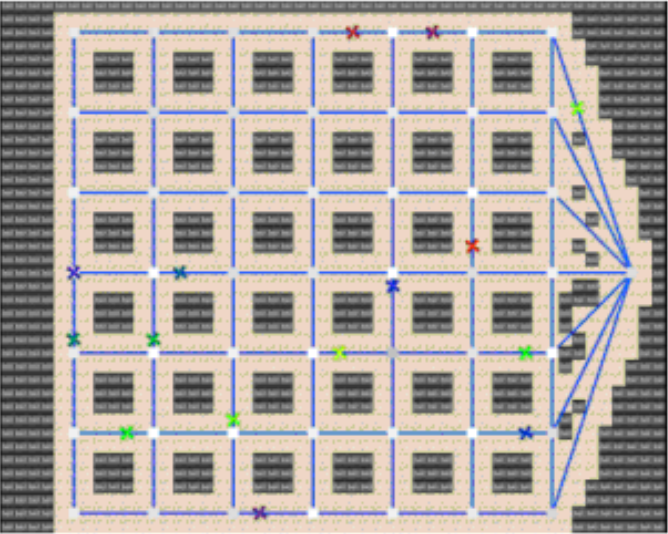
\includegraphics[width=0.9\linewidth]{images/mapa_grid.png}
		\label{fig:grid}
		\captionof*{figure}{Mapa \textit{grid}}
	\end{minipage}\hfill
	\begin{minipage}{0.5\textwidth}
		\centering
		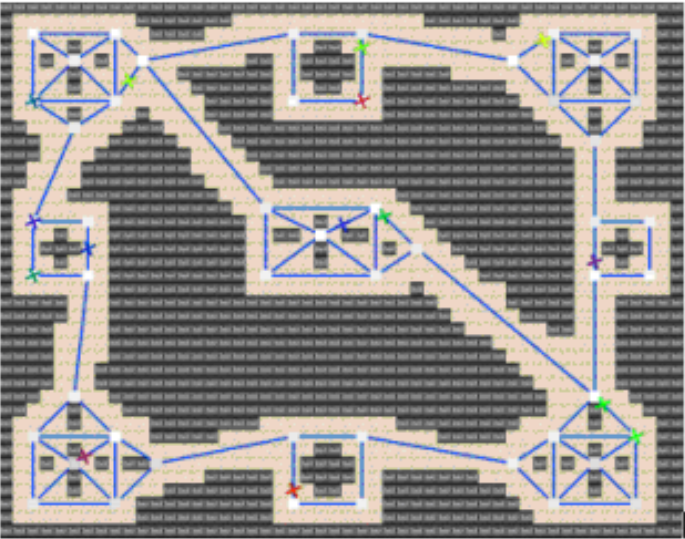
\includegraphics[width=0.9\linewidth]{images/mapa_ilhas.png}
		\label{fig:islands}
		\captionof*{figure}{Mapa \textit{islands}}
	\end{minipage}
	\begin{minipage}{0.5\textwidth}
		\centering
		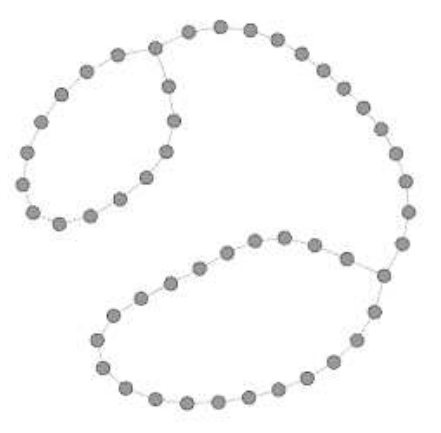
\includegraphics[width=\linewidth]{images/mapa_cicles_corridor.png}
		\label{fig:cicles_corridor}
		\captionof*{figure}{Mapa \textit{cicles corridor}}
	\end{minipage}
	\caption*{Fonte: \citep{sampaiophd}}
	\label{fig:mapas}
\end{figure}

Nas seções seguintes, serão discutidos os dois grupos de experimentos 
realizados. Eles foram chamados de Experimentos de \textit{Tuning} e de 
comparação.

\section{Experimentos de \textit{Tuning}}

\textit{Tuning} pode ser traduzido, do inglês, para ajuste. Esta seção tem como 
finalidade descrever e apresentar os resultados dos experimentos desenvolvidos 
para buscar o ajuste dos operadores que compõem as melhores heurísticas 
evolucionárias estudadas nesta pesquisa. Por exemplo, qual seria a melhor forma 
de inicializar um indivíduo? Existem ao todo doze formas diferentes de compor 
o operador de inicialização de indivíduos de uma heurística evolucionária 
utilizando os operadores propostos no \chapref{chp:abordagens}.

Primeiramente, foram realizados experimentos para determinar um número máximo 
de avaliações que permitisse distinguir os desempenhos das heurísticas nos 
demais experimentos. Enquanto o número máximo de avaliações variou entre 10 mil 
e 150 mil, os demais parâmetros permaneceram fixados:

\begin{itemize}
	\item Algoritmo utilizado: Estratégia Evolucionária $(\mu + \lambda)$
	\item Número de turnos: 2 mil
	\item Número de agentes: 5
	\item $\mu$: 30
	\item $\lambda$: 180
	\item Mapa: \textit{islands}
	\item Criação de indivíduos: \textit{Random Centering}, 
	\textit{Random Partitioning}, \textit{Random Path Building}
	\item Mutação: \textit{Half Add Half Sub Small Changes}
\end{itemize}

O resultado apontava que 30 mil avaliações eram suficientes para as 
estratégias evoluírem de soluções notadamente ruins para soluções ao ponto 
de convergir.

Depois, foram testados os tamanhos de população. Nos algoritmos genéticos, 
esse parâmetro diz respeito à quantidade de indivíduos a cada geração. 
Já nas estratégias evolucionárias existem dois parâmetros relacionados ao tamanho 
da população: $\mu$ e $\lambda$, como foi discorrido no \chapref{alg_evo}. Um 
experimento similar ao anterior foi realizado: as diferenças eram o número de 
avaliações agora fixado em 30 mil, mas com $\mu$ e $\lambda$ variando para as 
Estratégias Evolucionárias e o tamanho da população variando para o algoritmos 
genéticos. Todos os quatro algoritmos apresentados nesse trabalho foram testados 
individualmente. $\lambda$ e o tamanho da população variaram entre 72 e 180. 
$\mu$ variou entre $1/4$, $1/5$ e $1/6$ do valor de $\lambda$.

Os resultados obtido foram:
\begin{itemize}
	\item População de 96 indivíduos para o Algoritmo Genético
	\item População de 110 indivíduos para o Algoritmo Genético de Estado Estável
	\item $\mu = 18$ e $\lambda = 90$ para a Estratégia Evolucionária 
	$(\mu + \lambda)$
	\item $\mu = 26$ e $\lambda = 156$ para a Estratégia Evolucionária 
	$(\mu, \lambda)$
\end{itemize}

Assim como os algoritmos evolucionários, o operador \textit{Melhorar}, utilizado 
pelos operadores de mutação, também itera um número arbitrário de vezes. Também 
foram feitos experimentos para identificar qual o número de iterações que seria 
suficiente para causar melhoras significativas em soluções. O algoritmo 
evolucionário utilizado para estes testes foi a Estratégia Evolucionária 
$(\mu + \lambda)$, com $\mu = 18$ e $\lambda = 90$. Os demais parâmetros foram 
fixados com valores iguais ao experimento do máximo número de avaliações, 
enquanto que o número de iterações no \textit{loop} do operador 
\textit{melhorar} variou entre 0 e 100, pois já que o operador leva bastante 
tempo para calcular uma resposta, valores acima de 100 se mostraram 
impraticáveis. Os resultados mostraram que a partir de 5 iterações, não havia 
variação significativa na qualidade dos indivíduos encontrados.

Finalmente, o experimento de \textit{tuning} foi configurado com os parâmetros 
de número máximo de avaliações, número máximo de iterações no operador 
\textit{Melhorar} e o tamanho da população fixados (este 
último por algoritmo) nos valores acima reportados. O número de unidades de 
tempo em cada simulação foi mantido em 2mil. No entano, os mapas onde os agentes 
patrulham foram variados entre os três grafos apresentados na \figref{fig:mapas} 
e o tamanho da sociedade de agentes entre 1, 5, 10 e 15. Para cada um desses 
foram simuladas cada umas das composições de operadores e algoritmos. No final, 
seus respectivos valores da Média Quadrática dos Intervalos para o melhor 
indivíduo encontrado foram registrados.

Para comparar as estratégias, no entanto, foi utilizada a seguinte estratégia 
proposta por \citep{sampaiophd}. Os valores das médias quadráticas dos 
intervalos foram normalizadas, para que se tenha um único valor para todas as 
sociedades de agentes por heurística, por mapa. Esta medida é obtida através da 
multiplicação da média quadrática dos intervalos pelo tamanho da sociedade de 
agentes que o obteve (no caso desses experimentos, 1, 5, 10 e 15). Depois, esse 
valor é somado. Veja a equação abaixo:

$$MQIN = \sum MQI_{S} * |S|$$

Onde $S$ é a sociedade de agentes e $MQI_{S}$ é a Média Quadrática dos 
Intervalos obtida pela sociedade $S$.

Depois, foi elaborado um \textit{ranking}, para cada mapa, ordenado pela $MQIN$. 
Por fim, foi retirada uma média dos \textit{rankings} por heurística e as 5 
melhores estão listadas na \tabref{top5}.

\begin{table}
	\centering
	\caption{As 5 melhores heurísticas evolucionárias}
	\label{top5}
	\begin{tabularx}{\linewidth}{|X|X|X|X|X|X|}
		\hline
		\textbf{Algoritmo Evolucionário} & \textbf{Mutação} & \textbf{\textit{Centering}} & \textbf{\textit{Partitioning}} & \textbf{\textit{Path Building}} & \textbf{Ranking Médio} \\
		\hline
		Algoritmo Genético & \textit{Half Add Half Sub Small Changes} & \textit{Approximated Maximum Distance Centering} & \textit{Heuristic Graph Partitioning} & \textit{Nearest Neighbor Path Building} &  4,000\\
		\hline
		Algoritmo Genético de Estado Estável & \textit{Half Add Half Sub Small Changes} & \textit{Approximated Maximum Distance Centering} & \textit{Heuristic Graph Partitioning} & \textit{Nearest Neighbor Path Building} & 4,000\\
		\hline
		Algoritmo Genético de Estado Estável & \textit{Half Add Half Sub Small Changes} & \textit{Random Centering} & \textit{Heuristic Graph Partitioning} & \textit{Nearest Neighbor Path Building} & 5,333\\
		\hline
		Algoritmo Genético & \textit{Half Add Half Sub Small Changes} & \textit{Random Centering} & \textit{Heuristic Graph Partitioning} & \textit{Nearest Neighbor Path Building} & 5,666\\
		\hline
		Estratégia Evolucionária $(\mu, \lambda)$ & \textit{Half Add Half Sub Small Changes} & \textit{Approximated Maximum Distance Centering} & \textit{Heuristic Graph Partitioning} & \textit{Nearest Neighbor Path Building} & 8,333\\
		\hline
		%		\citep{Machado:2002:MPE:1765317.1765332} & Patrulha Multiagente "Padrão" & Simulação & Ociosidade instantânea do nó, ociosidade instantânea do grafo, ociosidade do grafo, ociosidade máxima e tempo de exploração \\
		%		\hline
	\end{tabularx}
	\caption*{Fonte: O autor}
\end{table}

Quatro das heurísticas presentes no \textit{top 5} são Algoritmos Genéticos, que 
utilizam o operador de recombinação (Estratégias Evolucionárias só utilizam 
Mutação). Este é um forte indício da eficácia do 
\textit{Simple Random Crossover} proposto nesta pesquisa.

Outra importante informação da \tabref{top5} é que, com exceção da 3ª e 4ª 
colocadas, as melhores heurísticas se valem dos operadores propostos no 
\chapref{chp:abordagens} que não são exclusivamente aleatórios, mas se valem de 
informações sobre o problema para computar suas respostas. Notoriamente, os 
operadores \textit{Approximated Maximum Distance Centering}, 
\textit{Heuristic Graph Partitioning} e \textit{Nearest Neighbor Path Building} 
obtiveram excelentes resultados.

Com esses resultados, as duas primeiras heurísticas da \tabref{top5} foram 
selecionadas para comparação com algoritmos propostos por outros autores.

\section{Experimentos de Comparação}

Para verificar a qualidade das heurísticas evolucionárias foram feitos 
experimentos comparando com as três melhores estratégias gravitacionais 
propostas por \citep{sampaiophd}. São elas: $grav(Node,Ar,2,sum)$, 
$grav(Node,Ar,1,max)$ e $grav(Edge,Ar,1,max)$.

Os experimentos de comparação colocaram cada estratégia para gerar quatro 
sociedades de agentes que patrulhassem os mapas ilustrados na 
\figref{fig:mapas}. O tamanho das sociedades variou entre 1, 5, 10 e 15, tal 
como nos experimentos de \textit{tuning}.

A \tabref{result_genetic} mostra os resultados obtidos pela heurística do 
Algoritmo Genético (1º lugar na \tabref{top5}). Enquanto que a 
\tabref{result_ssgenetic} mostra os resultados da heurística do Algoritmo 
Genético de Estado Estável. As tabelas~\ref{result_grav1}, ~\ref{result_grav2} 
e~\ref{result_grav3} mostram os resultados das estratégias gravitacionais 
$grav(Node,Ar,2,sum)$, $grav(Node,Ar,1,max)$ e $grav(Edge,Ar,1,max)$, respectivamente.

\begin{table}
	\centering
	\caption{Resultados do Algoritmo Genético}
	\label{result_genetic}
	\begin{tabularx}{\linewidth}{|X|X|X|X|X|}
		\hline
		\textbf{Algoritmo Genético} & \textbf{1 Agente} & \textbf{5 Agentes} & \textbf{10 Agentes} & \textbf{15 Agentes} \\
		\hline
		Mapa \textit{Cicles Corridor} & 150,007 & 32,834 & 17,445 & 11,561 \\
		\hline
		Mapa \textit{Grid} & 208,876 & 44,393 & 23,293 & 15,617 \\
		\hline
		Mapa \textit{Islands} & 188,480 & 38,340 & 16,179 & 10,619 \\
		\hline
		%		\citep{Machado:2002:MPE:1765317.1765332} & Patrulha Multiagente "Padrão" & Simulação & Ociosidade instantânea do nó, ociosidade instantânea do grafo, ociosidade do grafo, ociosidade máxima e tempo de exploração \\
		%		\hline
	\end{tabularx}
	\caption*{Fonte: O autor}
\end{table}

\begin{table}
	\centering
	\caption{Resultados do Algoritmo Genético de Estado Estável}
	\label{result_ssgenetic}
	\begin{tabularx}{\linewidth}{|X|X|X|X|X|}
		\hline
		\textbf{Algoritmo Genético de Estado Estável} & \textbf{1 Agente} & \textbf{5 Agentes} & \textbf{10 Agentes} & \textbf{15 Agentes} \\
		\hline
		Mapa \textit{Cicles Corridor} & 150,007 & 32,802 & 16,664 & 11,797 \\
		\hline
		Mapa \textit{Grid} & 208,876 & 44,240 & 23,416 & 15,652 \\
		\hline
		Mapa \textit{Islands} & 189,175 & 38,211 & 17,332 & 10,400 \\
		\hline
		%		\citep{Machado:2002:MPE:1765317.1765332} & Patrulha Multiagente "Padrão" & Simulação & Ociosidade instantânea do nó, ociosidade instantânea do grafo, ociosidade do grafo, ociosidade máxima e tempo de exploração \\
		%		\hline
	\end{tabularx}
	\caption*{Fonte: O autor}
\end{table}

\begin{table}
	\centering
	\caption{Resultados da Estratégia Gravitacional $grav(Node,Ar,2,sum)$}
	\label{result_grav1}
	\begin{tabularx}{\linewidth}{|X|X|X|X|X|}
		\hline
		\textbf{$grav$($Node$, $Ar$, $2$, $sum$)} & \textbf{1 Agente} & \textbf{5 Agentes} & \textbf{10 Agentes} & \textbf{15 Agentes} \\
		\hline
		Mapa \textit{Cicles Corridor} & 150,077 & 33,904 & 16,419 & 10,724 \\
		\hline
		Mapa \textit{Grid} & 223,844 & 45,966 & 22,777 & 15,023 \\
		\hline
		Mapa \textit{Islands} & 196,727 & 38,356 & 15,232 & 9,8 \\
		\hline
		%		\citep{Machado:2002:MPE:1765317.1765332} & Patrulha Multiagente "Padrão" & Simulação & Ociosidade instantânea do nó, ociosidade instantânea do grafo, ociosidade do grafo, ociosidade máxima e tempo de exploração \\
		%		\hline
	\end{tabularx}
	\caption*{Fonte: O autor}
\end{table}

\begin{table}
	\centering
	\caption{Resultados da Estratégia Gravitacional $grav(Node,Ar,1,max)$}
	\label{result_grav2}
	\begin{tabularx}{\linewidth}{|X|X|X|X|X|}
		\hline
		\textbf{$grav$($Node$, $Ar$, $1$, $max$)} & \textbf{1 Agente} & \textbf{5 Agentes} & \textbf{10 Agentes} & \textbf{15 Agentes} \\
		\hline
		Mapa \textit{Cicles Corridor} & 150,077 & 35,334 & 16,844 & 10,807 \\
		\hline
		Mapa \textit{Grid} & 210,857 & 46,483 & 22,803 & 15,076 \\
		\hline
		Mapa \textit{Islands} & 192,774 & 39,645 & 15,76 & 10,468 \\
		\hline
		%		\citep{Machado:2002:MPE:1765317.1765332} & Patrulha Multiagente "Padrão" & Simulação & Ociosidade instantânea do nó, ociosidade instantânea do grafo, ociosidade do grafo, ociosidade máxima e tempo de exploração \\
		%		\hline
	\end{tabularx}
	\caption*{Fonte: O autor}
\end{table}

\begin{table}
	\centering
	\caption{Resultados da Estratégia Gravitacional $grav(Edge,Ar,1,max)$}
	\label{result_grav3}
	\begin{tabularx}{\linewidth}{|X|X|X|X|X|}
		\hline
		\textbf{$grav$($Edge$, $Ar$, $1$, $max$)} & \textbf{1 Agente} & \textbf{5 Agentes} & \textbf{10 Agentes} & \textbf{15 Agentes} \\
		\hline
		Mapa \textit{Cicles Corridor} & 150,077 & 46,444 & 21,995 & 11,553 \\
		\hline
		Mapa \textit{Grid} & 208,516 & 51,816 & 24,084 & 16,073 \\
		\hline
		Mapa \textit{Islands} & 187,758 & 56,707 & 15,701 & 10,417 \\
		\hline
		%		\citep{Machado:2002:MPE:1765317.1765332} & Patrulha Multiagente "Padrão" & Simulação & Ociosidade instantânea do nó, ociosidade instantânea do grafo, ociosidade do grafo, ociosidade máxima e tempo de exploração \\
		%		\hline
	\end{tabularx}
	\caption*{Fonte: O autor}
\end{table}

Um resultado inesperado foi o baixo desempenho da estratégia \textit{Single Cycle} para um 
único agente no mapa de \textit{grid}, já que está é tida, na literatura, como 
a solução mais próxima da ótima, para um único agente com a métrica de Intervalo 
Máximo. Nesses experimentos, para a métrica de média quadrática dos intervalos a 
estratégia de ciclo único obteve o pior resultado no mapa de \textit{grid}. No 
entanto, para o mapa de \textit{Cicles Corridor}, a \textit{Single Cycle} foi 
melhor em todos os tamanhos de sociedade.

As duas heurísticas evolucionárias tiveram um desempenho muito similar em 
todos os experimentos, algo que já tinha sido observado quando elas obtiveram 
o mesmo ranking médio nos experimentos de \textit{tuning}. Elas ficaram muito 
próximas dos melhores resultados para sociedades de tamanho 1 e 5 em todos os 
mapas, chegando, inclusive, a superar as estratégias \textit{Single Cycle}, 
$grav(Node,Ar,2,sum)$ e $grav(Node,Ar,1,max)$ nos mapas de \textit{grid} e 
\textit{islands}.

Os gráficos das figuras~\ref{fig:graph_agentes1}, ~\ref{fig:graph_agentes2}, 
~\ref{fig:graph_agentes3} e~\ref{fig:graph_agentes4} abaixo ajudam a 
compreender melhor os resultados encontrados.

\begin{figure}[b]
	\caption[Resultado para sociedade de tamanho 1]{Resultado para sociedade 
		de tamanho 1}
	\centering
	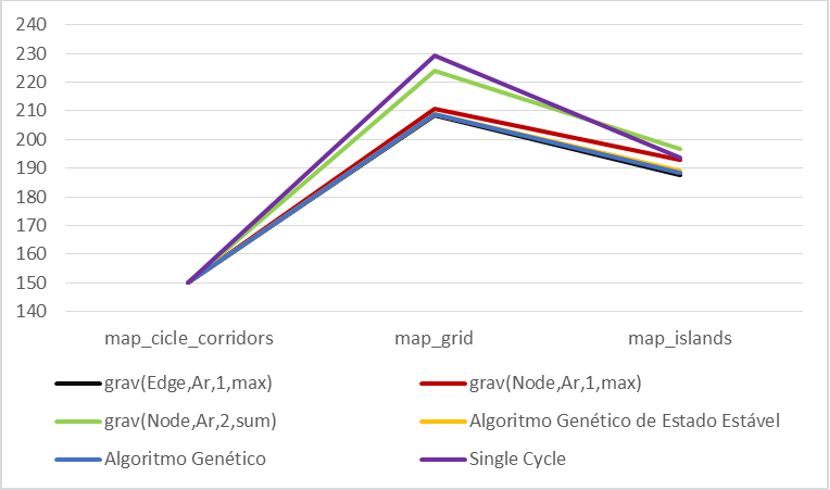
\includegraphics[width=\columnwidth]{images/graph_agent1.png}
	\caption*{Fonte: O Autor}
	\label{fig:graph_agentes1}
\end{figure}

\begin{figure}
	\caption[Resultado para sociedade de tamanho 5]{Resultado para sociedade 
		de tamanho 5}
	\centering
	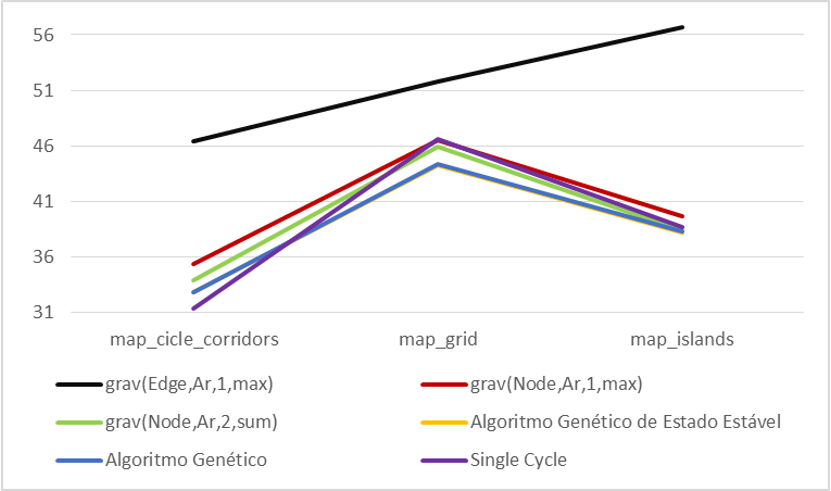
\includegraphics[width=\columnwidth]{images/graph_agent2.png}
	\caption*{Fonte: O Autor}
	\label{fig:graph_agentes2}
\end{figure}

\begin{figure}
	\caption[Resultado para sociedade de tamanho 10]{Resultado para sociedade 
		de tamanho 10}
	\centering
	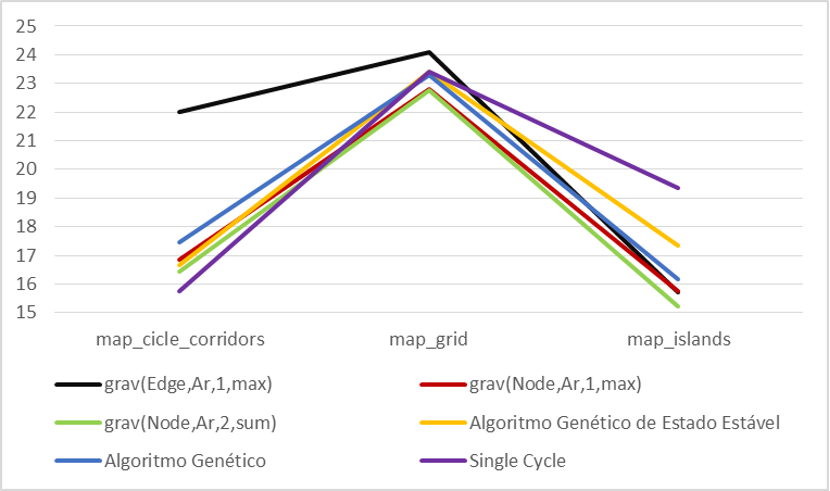
\includegraphics[width=\columnwidth]{images/graph_agent3.png}
	\caption*{Fonte: O Autor}
	\label{fig:graph_agentes3}
\end{figure}

\begin{figure}
	\caption[Resultado para sociedade de tamanho 15]{Resultado para sociedade 
		de tamanho 15}
	\centering
	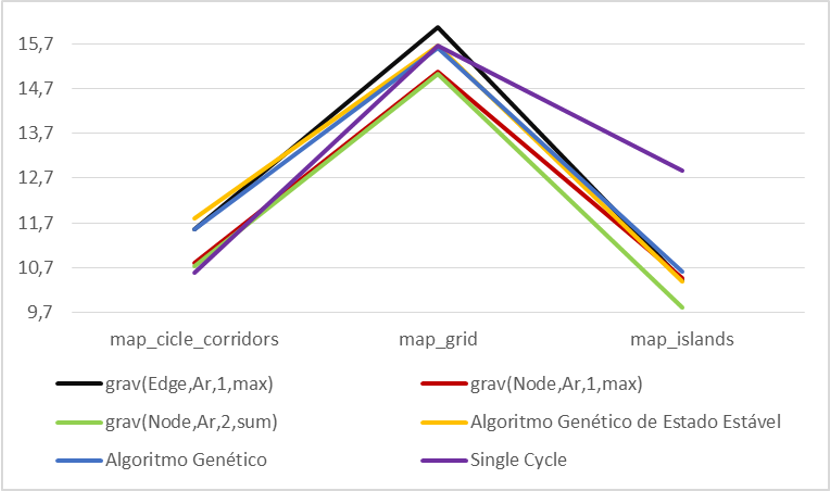
\includegraphics[width=\columnwidth]{images/graph_agent4.png}
	\caption*{Fonte: O Autor}
	\label{fig:graph_agentes4}
\end{figure}